\documentclass[aspectratio=169,11pt]{beamer}

% -----------------------------------------------------------------------------
% Minimalist, Professional Software Architecture Theme
% -----------------------------------------------------------------------------
\usetheme{default}
\usefonttheme{structurebold}

% Typography & Encoding
\usepackage[utf8]{inputenc}
\usepackage[T1]{fontenc}
\usepackage{lmodern}
\usepackage{inconsolata}
\usepackage{tikz}
\usetikzlibrary{arrows.meta, positioning, shapes.geometric, fit, backgrounds, calc}
\usepackage{booktabs}

% Single Restrained Accent Color (Navy) & Slate Text
\definecolor{textMain}{RGB}{15, 23, 42}         % Slate 900
\definecolor{textMuted}{RGB}{71, 85, 105}       % Slate 600
\definecolor{accentNavy}{RGB}{29, 78, 216}      % Blue 700
\definecolor{boxBg}{RGB}{248, 250, 252}         % Slate 50
\definecolor{lineColor}{RGB}{203, 213, 225}     % Slate 300

\setbeamercolor{background canvas}{bg=white}
\setbeamercolor{normal text}{fg=textMain}
\setbeamercolor{frametitle}{fg=accentNavy, bg=white}
\setbeamercolor{title}{fg=accentNavy}
\setbeamercolor{subtitle}{fg=textMuted}
\setbeamercolor{item}{fg=accentNavy}
\setbeamercolor{subitem}{fg=textMuted}
\setbeamercolor{block title}{fg=accentNavy, bg=boxBg}
\setbeamercolor{block body}{fg=textMain, bg=white}

% Strict slide margins and padding to prevent vertical/horizontal overflow
\setbeamersize{text margin left=0.8cm, text margin right=0.8cm}
\setbeamertemplate{navigation symbols}{}

\setbeamertemplate{frametitle}{
  \vspace{0.25cm}
  \noindent{\large\textbf{\color{accentNavy}\insertframetitle}}
  \par\vspace{0.04cm}
  \noindent{\color{lineColor}\rule{\textwidth}{0.6pt}}
  \vspace{0.1cm}
}

\setbeamertemplate{footline}{
  \hfill\usebeamerfont{page number in head/foot}\color{textMuted}\insertframenumber{} / \inserttotalframenumber\hspace*{0.8cm}\vspace{0.3cm}
}

% -----------------------------------------------------------------------------
% Title Information
% -----------------------------------------------------------------------------
\title{\textbf{Autonomous Code Review Agent}}
\subtitle{Architecture, Deterministic Intelligence \& Multi-Agent Review Workflow}
\author{Engineering Architecture Review}
\institute{Autonomous Review Platform}
\date{\today}

\begin{document}

% -----------------------------------------------------------------------------
% SLIDE 1: Title Slide
% -----------------------------------------------------------------------------
\begin{frame}[plain]
  \vspace{1.0cm}
  {\Large\textbf{\color{accentNavy}Autonomous Code Review Agent}}
  
  \vspace{0.25cm}
  {\normalsize\color{textMuted}Evidence-Driven, Multi-Agent Pull Request Review Platform with Sandboxed Verification}
  
  \vspace{0.5cm}
  \noindent{\color{lineColor}\rule{0.35\textwidth}{1pt}}
  
  \vspace{0.35cm}
  {\footnotesize\textbf{System Architecture \& Technical Deep Dive}}
  
  \vspace{0.35cm}
  {\footnotesize\color{textMuted}Repository: \href{https://github.com/AyushPrakash414/Autonomous-Code-Review-Agent}{\color{accentNavy}\texttt{https://github.com/AyushPrakash414/Autonomous-Code-Review-Agent}}}
\end{frame}

% -----------------------------------------------------------------------------
% SLIDE 2: Problem Statement
% -----------------------------------------------------------------------------
\begin{frame}{1. Problem Statement \& Industry Gaps}
  \textbf{Traditional Automated Review Tools Fall Short:}
  \vspace{0.25cm}
  \begin{itemize}
    \item \textbf{Syntax Linters (Checkstyle, SonarQube, ESLint):}
      \begin{itemize}
        \item Surface syntax, style, and formatting violations.
        \item Lack semantic understanding of cross-module architecture and behavior.
      \end{itemize}
    \vspace{0.25cm}
    \item \textbf{Generic LLM Review Bots:}
      \begin{itemize}
        \item Execute a monolithic prompt for every PR regardless of relevance.
        \item Hallucinate file paths, dependencies, and false security warnings.
        \item Suggest mock test snippets without ever compiling or verifying them.
      \end{itemize}
    \vspace{0.25cm}
    \item \textbf{High Developer Noise:} Developers ignore unverified AI comments.
  \end{itemize}
\end{frame}

% -----------------------------------------------------------------------------
% SLIDE 3: Core Objective & Solution
% -----------------------------------------------------------------------------
\begin{frame}{2. Project Objective: The Senior Reviewer Paradigm}
  \textbf{Review PRs with the rigor and empirical validation of a Senior Staff Engineer:}
  \vspace{0.25cm}
  \begin{itemize}
    \item \textbf{Deterministic First, LLM Second:}
      \begin{itemize}
        \item Extract ASTs, call-graphs, and diffs statically before AI reasoning.
      \end{itemize}
    \vspace{0.2cm}
    \item \textbf{Explainable Capability Routing:}
      \begin{itemize}
        \item Only invoke relevant specialist agents based on quantifiable code signals.
      \end{itemize}
    \vspace{0.2cm}
    \item \textbf{Sandboxed Test Execution:}
      \begin{itemize}
        \item Generated regression tests compile and run inside Docker sandboxes.
      \end{itemize}
    \vspace{0.2cm}
    \item \textbf{Empirical Verification:}
      \begin{itemize}
        \item Challenge findings against repository facts to eliminate false positives.
      \end{itemize}
  \end{itemize}
\end{frame}

% -----------------------------------------------------------------------------
% SLIDE 4: High-Level System Architecture
% -----------------------------------------------------------------------------
\begin{frame}{3. High-Level System Architecture}
  \centering
  \vspace{-0.1cm}
  \resizebox{0.92\textwidth}{!}{
  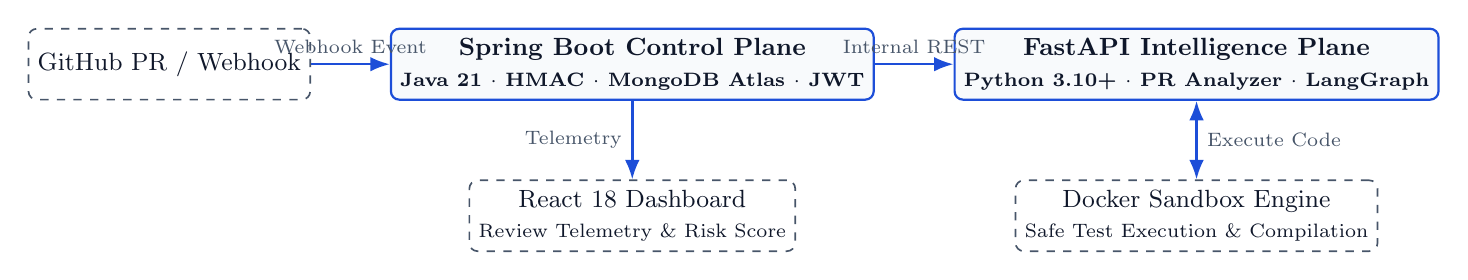
\begin{tikzpicture}[
    node distance=0.8cm and 1.2cm,
    box/.style={rectangle, draw=accentNavy, text=textMain, fill=boxBg, rounded corners=3pt, minimum width=3.2cm, minimum height=0.9cm, font=\small\bfseries, align=center, line width=0.8pt},
    ext/.style={rectangle, draw=textMuted, text=textMain, fill=white, rounded corners=3pt, minimum width=2.6cm, minimum height=0.9cm, font=\small, align=center, line width=0.6pt, dashed}
  ]
    % Primary Flow Nodes
    \node[ext] (gh) {GitHub PR / Webhook};
    \node[box, right=1.0cm of gh] (control) {Spring Boot Control Plane\\{\scriptsize Java 21 $\cdot$ HMAC $\cdot$ MongoDB Atlas $\cdot$ JWT}};
    \node[box, right=1.0cm of control] (intel) {FastAPI Intelligence Plane\\{\scriptsize Python 3.10+ $\cdot$ PR Analyzer $\cdot$ LangGraph}};

    % Downstream Nodes
    \node[ext, below=1.0cm of control] (dash) {React 18 Dashboard\\{\scriptsize Review Telemetry \& Risk Score}};
    \node[ext, below=1.0cm of intel] (box) {Docker Sandbox Engine\\{\scriptsize Safe Test Execution \& Compilation}};

    % Directional Connectors with clear spacing
    \draw[-{Latex[scale=1.0]}, line width=0.9pt, draw=accentNavy] (gh) -- node[above, font=\scriptsize\color{textMuted}] {Webhook Event} (control);
    \draw[-{Latex[scale=1.0]}, line width=0.9pt, draw=accentNavy] (control) -- node[above, font=\scriptsize\color{textMuted}] {Internal REST} (intel);
    \draw[-{Latex[scale=1.0]}, line width=0.9pt, draw=accentNavy] (control) -- node[left, font=\scriptsize\color{textMuted}] {Telemetry} (dash);
    \draw[{Latex[scale=1.0]}-{Latex[scale=1.0]}, line width=0.9pt, draw=accentNavy] (intel) -- node[right, font=\scriptsize\color{textMuted}] {Execute Code} (box);
  \end{tikzpicture}
  }

  \vspace{0.4cm}
  \begin{itemize}
    \item \textbf{Control Plane:} Webhook ingestion, lifecycle management, and persistence.
    \item \textbf{Intelligence Plane:} Code parsing, routing, LangGraph agents, and verification.
    \item \textbf{Isolation Boundary:} Untrusted repository and AI code never runs on host.
  \end{itemize}
\end{frame}

% -----------------------------------------------------------------------------
% SLIDE 5: Control Plane Responsibilities
% -----------------------------------------------------------------------------
\begin{frame}{4. Control Plane Responsibilities (Spring Boot 3)}
  \textbf{Enterprise Foundation \& Review Lifecycle Management:}
  \vspace{0.25cm}
  \begin{itemize}
    \item \textbf{Authentication \& Access Control:}
      \begin{itemize}
        \item Spring Security 6 stateless filter chain with JWT verification.
        \item MongoDB Atlas document storage for user profiles and roles.
      \end{itemize}
    \vspace{0.2cm}
    \item \textbf{Webhook Integrity:}
      \begin{itemize}
        \item Cryptographic HMAC-SHA256 signature verification on GitHub events.
      \end{itemize}
    \vspace{0.2cm}
    \item \textbf{Idempotent Review Lifecycle:}
      \begin{itemize}
        \item State machine: \texttt{\small QUEUED $\rightarrow$ ANALYZING $\rightarrow$ ROUTING $\rightarrow$ REVIEWING $\rightarrow$ COMPLETED}.
        \item Prevents duplicate review runs or duplicate comments on identical commits.
      \end{itemize}
    \vspace{0.2cm}
    \item \textbf{GitHub Publisher:} Publishes final inline comments and status checks.
  \end{itemize}
\end{frame}

% -----------------------------------------------------------------------------
% SLIDE 6: Intelligence Plane Responsibilities
% -----------------------------------------------------------------------------
\begin{frame}{5. Intelligence Plane Responsibilities (FastAPI)}
  \textbf{Deterministic Analysis \& Agent Orchestration:}
  \vspace{0.25cm}
  \begin{itemize}
    \item \textbf{Deterministic PR Analyzer:}
      \begin{itemize}
        \item Parses ASTs, classes, functions, and import trees.
        \item Emits \texttt{PRAnalysisReport} containing signals (e.g., dynamic SQL, layer changes).
      \end{itemize}
    \vspace{0.2cm}
    \item \textbf{Capability-Based Agent Router:}
      \begin{itemize}
        \item Matches PR signals against agent capabilities with weighted scoring.
        \item Produces an explainable \texttt{AgentExecutionPlan} (\texttt{RUN}, \texttt{SKIP}, \texttt{CONDITIONAL}).
      \end{itemize}
    \vspace{0.2cm}
    \item \textbf{LangGraph Review Workflow:}
      \begin{itemize}
        \item Manages shared state, parallel agent dispatch, and conditional verification.
      \end{itemize}
  \end{itemize}
\end{frame}

% -----------------------------------------------------------------------------
% SLIDE 7: Four Specialist Review Agents
% -----------------------------------------------------------------------------
\begin{frame}{6. Specialist Review Agents (MVP Scope)}
  \textbf{Four Core Agents with Strictly Bounded Responsibilities:}
  \vspace{0.25cm}
  \begin{itemize}
    \item \textbf{1. Security Agent:}
      \begin{itemize}
        \item OWASP vulnerabilities (SQLi, XSS, CSRF, SSRF, authentication flaws, secrets).
      \end{itemize}
    \vspace{0.15cm}
    \item \textbf{2. Architecture Agent:}
      \begin{itemize}
        \item Layer boundaries (e.g., Controller $\rightarrow$ Service $\rightarrow$ Repository), circular dependencies.
      \end{itemize}
    \vspace{0.15cm}
    \item \textbf{3. Test Agent (Active Validation):}
      \begin{itemize}
        \item Maps changed symbols to existing tests, identifies missing test coverage.
        \item Generates and compiles unit tests inside isolated Docker sandbox.
      \end{itemize}
    \vspace{0.15cm}
    \item \textbf{4. Code Quality Agent:}
      \begin{itemize}
        \item Cyclomatic complexity, maintainability, code smells, naming standards.
      \end{itemize}
  \end{itemize}
\end{frame}

% -----------------------------------------------------------------------------
% SLIDE 8: Detailed Agent Execution Flow Diagram
% -----------------------------------------------------------------------------
\begin{frame}{7. Agent Execution Flow}
  \centering
  \vspace{-0.1cm}
  \resizebox{0.88\textwidth}{!}{
  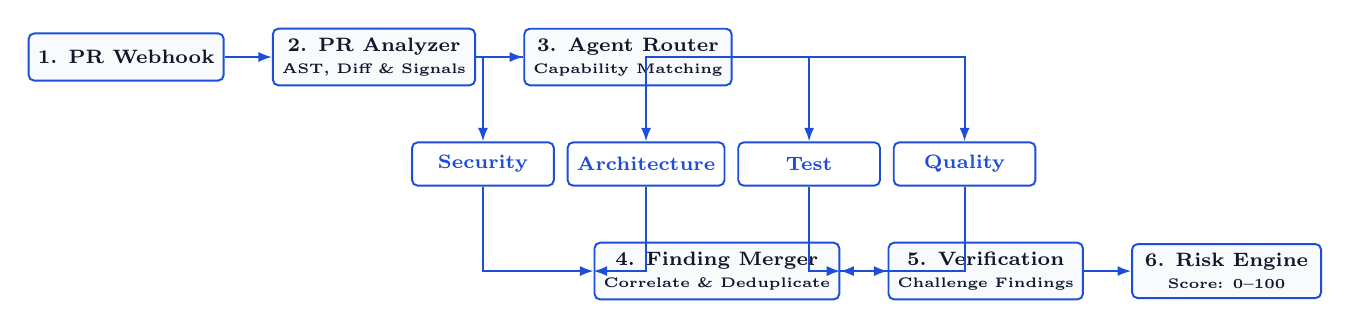
\begin{tikzpicture}[
    node distance=0.6cm and 0.8cm,
    stepNode/.style={rectangle, draw=accentNavy, text=textMain, fill=boxBg, rounded corners=2pt, minimum width=2.4cm, minimum height=0.6cm, font=\scriptsize\bfseries, align=center, line width=0.7pt},
    agentNode/.style={rectangle, draw=accentNavy, text=accentNavy, fill=white, rounded corners=2pt, minimum width=1.8cm, minimum height=0.55cm, font=\scriptsize\bfseries, align=center, line width=0.7pt}
  ]
    % Phase 1: Ingestion & Analysis
    \node[stepNode] (req) {1. PR Webhook};
    \node[stepNode, right=0.6cm of req] (pra) {2. PR Analyzer\\{\tiny AST, Diff \& Signals}};
    \node[stepNode, right=0.6cm of pra] (rtr) {3. Agent Router\\{\tiny Capability Matching}};

    % Phase 2: Parallel Specialist Agents
    \node[agentNode, below left=0.7cm and -0.4cm of rtr] (sec) {Security};
    \node[agentNode, right=0.15cm of sec] (arch) {Architecture};
    \node[agentNode, right=0.15cm of arch] (tst) {Test};
    \node[agentNode, right=0.15cm of tst] (qual) {Quality};

    % Phase 3: Synthesis & Verification
    \node[stepNode, below=0.7cm of arch, xshift=0.9cm] (mrg) {4. Finding Merger\\{\tiny Correlate \& Deduplicate}};
    \node[stepNode, right=0.6cm of mrg] (ver) {5. Verification\\{\tiny Challenge Findings}};
    \node[stepNode, right=0.6cm of ver] (rsk) {6. Risk Engine\\{\tiny Score: 0--100}};

    % Clean, uncrossed connections
    \draw[-{Latex[scale=0.8]}, line width=0.7pt, draw=accentNavy] (req) -- (pra);
    \draw[-{Latex[scale=0.8]}, line width=0.7pt, draw=accentNavy] (pra) -- (rtr);

    \draw[-{Latex[scale=0.8]}, line width=0.7pt, draw=accentNavy] (rtr) -| (sec);
    \draw[-{Latex[scale=0.8]}, line width=0.7pt, draw=accentNavy] (rtr) -| (arch);
    \draw[-{Latex[scale=0.8]}, line width=0.7pt, draw=accentNavy] (rtr) -| (tst);
    \draw[-{Latex[scale=0.8]}, line width=0.7pt, draw=accentNavy] (rtr) -| (qual);

    \draw[-{Latex[scale=0.8]}, line width=0.7pt, draw=accentNavy] (sec) |- (mrg);
    \draw[-{Latex[scale=0.8]}, line width=0.7pt, draw=accentNavy] (arch) |- (mrg);
    \draw[-{Latex[scale=0.8]}, line width=0.7pt, draw=accentNavy] (tst) |- (mrg);
    \draw[-{Latex[scale=0.8]}, line width=0.7pt, draw=accentNavy] (qual) |- (mrg);

    \draw[-{Latex[scale=0.8]}, line width=0.7pt, draw=accentNavy] (mrg) -- (ver);
    \draw[-{Latex[scale=0.8]}, line width=0.7pt, draw=accentNavy] (ver) -- (rsk);
  \end{tikzpicture}
  }

  \vspace{0.35cm}
  \begin{itemize}
    \item \textbf{Dynamic Branching:} LangGraph skips irrelevant agents according to plan.
    \item \textbf{Deduplication:} Multiple agents flagging the same issue are consolidated.
  \end{itemize}
\end{frame}

% -----------------------------------------------------------------------------
% SLIDE 9: Finding Verification & Deterministic Risk Engine
% -----------------------------------------------------------------------------
\begin{frame}{8. Finding Verification \& Risk Analysis}
  \textbf{Eliminating False Positives \& Quantifying Review Risk:}
  \vspace{0.25cm}
  \begin{itemize}
    \item \textbf{Finding Verification Engine:}
      \begin{itemize}
        \item Challenges candidate findings before publication to eliminate false alarms.
        \item Triages into explicit statuses: \texttt{\small VERIFIED}, \texttt{\small FALSE\_POSITIVE}, \texttt{\small UNCERTAIN}.
        \item Uses static confirmation and test reproductions.
      \end{itemize}
    \vspace{0.25cm}
    \item \textbf{Deterministic Risk Engine (Score 0--100):}
      \begin{itemize}
        \item Computed via deterministic scoring model:
        \item Factors: Verified Severity + Code Change Impact + Security Sensitivity + Missing Test Ratio.
        \item Categorized into: \texttt{\small LOW (0-30)}, \texttt{\small MEDIUM (31-60)}, \texttt{\small HIGH (61-85)}, \texttt{\small CRITICAL (86-100)}.
      \end{itemize}
  \end{itemize}
\end{frame}

% -----------------------------------------------------------------------------
% SLIDE 10: Core Design Principles
% -----------------------------------------------------------------------------
\begin{frame}{9. Core Design Principles}
  \textbf{Fundamental Rules Enforced Across the Platform:}
  \vspace{0.25cm}
  \begin{itemize}
    \item \textbf{Deterministic First, LLM Second:}
      \begin{itemize}
        \item Deterministic tools handle ASTs, line numbers, symbols, and dependencies.
        \item LLMs provide semantic reasoning, explanation, and ambiguity resolution.
      \end{itemize}
    \vspace{0.2cm}
    \item \textbf{Evidence Over Claims:}
      \begin{itemize}
        \item Every finding contains verifiable proof (diff lines, AST paths, or execution logs).
      \end{itemize}
    \vspace{0.2cm}
    \item \textbf{No Fake Implementations:}
      \begin{itemize}
        \item No placeholder methods or mocked results in production paths.
      \end{itemize}
    \vspace{0.2cm}
    \item \textbf{Sandboxed Untrusted Execution:}
      \begin{itemize}
        \item Untrusted repository code and AI-generated tests execute in isolated containers.
      \end{itemize}
  \end{itemize}
\end{frame}

% -----------------------------------------------------------------------------
% SLIDE 11: Key Technical Decisions & Rationale
% -----------------------------------------------------------------------------
\begin{frame}{10. Technical Decisions \& Rationale}
  \textbf{Technology Choices Aligned to Domain Requirements:}
  \vspace{0.25cm}
  \begin{itemize}
    \item \textbf{Spring Boot 3 + Java 21 (Control Plane):}
      \begin{itemize}
        \item Strong enterprise security (Spring Security 6, JWT, HMAC verification).
        \item Type-safe persistence and resilient webhook state lifecycle management.
      \end{itemize}
    \vspace{0.2cm}
    \item \textbf{FastAPI + Python 3.10+ (Intelligence Plane):}
      \begin{itemize}
        \item Rich AST parser ecosystem (Tree-sitter, ast) and native LangGraph integration.
      \end{itemize}
    \vspace{0.2cm}
    \item \textbf{MongoDB Atlas Persistence:}
      \begin{itemize}
        \item Flexible document schema for heterogeneous AST reports, review graphs, and findings.
      \end{itemize}
    \vspace{0.2cm}
    \item \textbf{LLM Provider Abstraction:}
      \begin{itemize}
        \item Common interface supporting Gemini, Ollama, and OpenAI via configuration.
      \end{itemize}
  \end{itemize}
\end{frame}

% -----------------------------------------------------------------------------
% SLIDE 12: Concrete Execution Walkthrough (Part 1)
% -----------------------------------------------------------------------------
\begin{frame}{11. End-to-End Walkthrough: Ingestion \& Routing}
  \textbf{Step-by-Step Scenario: Developer modifies Payment API}
  \vspace{0.25cm}
  \begin{enumerate}
    \item \textbf{PR Event:}
      \begin{itemize}
        \item Developer updates \texttt{PaymentController.java} \& \texttt{PaymentService.java}.
      \end{itemize}
    \vspace{0.15cm}
    \item \textbf{Webhook Ingestion:}
      \begin{itemize}
        \item Spring Boot validates HMAC-SHA256 signature and records PR revision.
      \end{itemize}
    \vspace{0.15cm}
    \item \textbf{Deterministic PR Analysis:}
      \begin{itemize}
        \item PR Analyzer detects public method changes and SQL query string concatenation.
      \end{itemize}
    \vspace{0.15cm}
    \item \textbf{Capability-Based Routing Decision:}
      \begin{itemize}
        \item \textbf{Security Agent (RUN | 94):} Triggered by dynamic SQL pattern \& auth annotations.
        \item \textbf{Architecture Agent (RUN | 88):} Controller-to-Service layer boundary change.
        \item \textbf{Test Agent (RUN | 92):} Public method modified with missing test coverage.
        \item \textbf{Quality Agent (RUN | 80):} High complexity code block detected.
      \end{itemize}
  \end{enumerate}
\end{frame}

% -----------------------------------------------------------------------------
% SLIDE 13: Concrete Execution Walkthrough (Part 2)
% -----------------------------------------------------------------------------
\begin{frame}{12. End-to-End Walkthrough: Verification \& Publishing}
  \textbf{Step-by-Step Scenario: Execution, Testing \& Publication}
  \vspace{0.25cm}
  \begin{enumerate}
    \setcounter{enumi}{4}
    \item \textbf{Parallel Agent Execution:}
      \begin{itemize}
        \item Security Agent identifies potential SQL Injection on line 42.
        \item Architecture Agent verifies clean Controller $\rightarrow$ Service layering.
      \end{itemize}
    \vspace{0.15cm}
    \item \textbf{Sandboxed Test Execution (Docker):}
      \begin{itemize}
        \item Test Agent generates unit tests for \texttt{PaymentService}.
        \item Compiles and runs test suite in Docker sandbox $\rightarrow$ Result: \textbf{\texttt{\small PASSED}}.
      \end{itemize}
    \vspace{0.15cm}
    \item \textbf{Finding Verification \& Risk Analysis:}
      \begin{itemize}
        \item Verification confirms SQL injection via AST data-flow trace $\rightarrow$ \textbf{\texttt{\small VERIFIED}}.
        \item Risk Engine calculates PR Risk Score = \textbf{84 / 100 (HIGH)}.
      \end{itemize}
    \vspace{0.15cm}
    \item \textbf{Publication:}
      \begin{itemize}
        \item Spring Boot posts inline review comments to GitHub and updates Dashboard.
      \end{itemize}
  \end{enumerate}
\end{frame}

% -----------------------------------------------------------------------------
% SLIDE 14: Summary Slide
% -----------------------------------------------------------------------------
\begin{frame}{13. Summary \& Engineering Value}
  \textbf{What Makes the Autonomous Code Review Agent Distinct:}
  \vspace{0.3cm}
  \begin{itemize}
    \item \textbf{High Precision, Low Noise:} Capability routing and empirical verification eliminate false alarms.
    \vspace{0.25cm}
    \item \textbf{Proven Test Adequacy:} Generated tests are actually compiled and executed in Docker.
    \vspace{0.25cm}
    \item \textbf{Deterministic Risk:} Objective 0--100 risk score and code change impact calculation.
    \vspace{0.25cm}
    \item \textbf{Production Architecture:} Decoupled Spring Boot control plane and FastAPI intelligence plane.
  \end{itemize}
  \vspace{0.5cm}
  \centering
  {\color{accentNavy}\textbf{Evidence Over Claims. Deterministic First, LLM Second.}}
\end{frame}

\end{document}
